\section{Implicit navigation in vEB layout}
Consider $N = 2^h - 1$ keys where $h$ is a power of 2, and the implicit cache-oblivious vEB layout of their corresponding complete binary tree, where the keys are suitably permuted and stored in an array of length $N$ without using pointers (as it happens in the classical implicit binary heap but the rule here is different). The root is in the first position of the array. Find a rule that, given the position of the current node, it is possible to locate in the array the positions of its left and right children. Discuss how to apply this layout to obtain (a) a static binary search tree and (b) a heap data structure, discussing the cache complexity.

\vspace{0.5cm}
\subsection{Solution.} We assume that the keys are stored in a zero-indexed array $T$. Given and index $0 \leq i < T.length$ we will give a rule for computing the index of its children.

\begin{center}
  \begin{tikzpicture}[sibling distance=10pt]
    \tikzstyle{every node}=[circle,draw]
    \Tree [.0 [.1 [.3 [.4 ]  [.5 ] ] [.6 [.7 ] [.8 ] ] ] [.2 [.9 [.10 ] [.11 ] ] [.12 [.13 ] [.14 ] ] ] ]
  \end{tikzpicture}
\end{center}

As  by hypothesis, we'll assume $H = 2^k, k \in \mathcal{Z} \setminus \{0, 1\} $.
\label{15_shift_layouts}~\paragraph{Shifted layouts} We start by introducing the notion of \emph{shifted layout}: a \emph{shifted layout L'} of a layout \emph{L} is a layout of the same size whose \emph{a} root is shifted from the one of \emph{L} of an offset \emph{g}:
	\begin{equation}
	\textsc{height(L)} == \textsc{height(L')}, L'.root = L.root + a
	\end{equation}

Then
	\begin{equation}
	n \in L, n' \in L': n.index == n'.index \to n'.position == n.position + a \forall n \in L, n' \in L'
	\end{equation}
Trivially, as the two layouts are shifted in the root, the same shift is propagated to the remaining nodes in the layout.

\label{15_odd_levels_contiguity}~\paragraph{Contiguous children} Given a layout \emph{L}, we are able to \emph{cut} it until we reach a base case of layout \emph{L'} of height $2$ and root \emph{a}.
It is trivial to see as this is populated as the following shows:
	\begin{center}
	\begin{tikzpicture}[sibling distance=10pt]
	\Tree [.a [.a+1 ] [.a+2 ] ]
	\end{tikzpicture}
	\end{center}
by the definition of base case for the \emph{vEB construction}.
Then, provided we know to be in the \emph{a} index we are able to answer trivially with
	\begin{gather*} \label{15_contiguity}
	\textsc{LEFT(a)} = a + 1	\\
	\textsc{RIGHT(a)} = a + 2	\\
	\end{gather*}

\label{15_even_levels_gap}~\paragraph{Non-contiguous children} Given a layout \emph{L}, we are able to \emph{cut} it until we reach a base case of
	\begin{center}
	\begin{tikzpicture}[sibling distance=10pt]
	\Tree [.a
	[.a+1
		[.{$a+\gamma_a$} [.{$a+\gamma_a + 1$} ]  [.{$a+\gamma_a + 2$} ] ]
		[.{$a+\gamma_a + S$} [.{$a+\gamma_a + S + 1$} ] [.{$a+\gamma_a + S + 2$} ] ] ]
	[.a+2
		[.{$a+\gamma_a + 2 \cdot S$} [.{$\dots$} ] [.{$\dots$} ] ] [.{$a+\gamma_a + 3 \cdot S$} [.{$\dots$} ] 
	[.{$\dots$} ] ] ] ]
	\end{tikzpicture}
	\end{center}
The first two levels are trivial by \ref{15_even_levels_gap}.
From the second to the third we find instead a jump $\gamma_a$.
By construction of the \emph{layout} the position $a + \gamma_a$ is populated right after $a + 2$: in this trivial case we have a jump of size $2$.
This holds also for $a + \gamma_a + S$, as it is populated right after $a + \gamma_a + 2$ and so on and so forth on the same level.
Given that \emph{height(T)} $= 4$ we have jumps $\gamma_a = 2$: this does not hold for any height: let $H = 2h$ be the height of a \emph{vEB tree} s.t. $h > 1$, $a$ be a node at level $h + 1$, $b$ be a node at level $l \not h +1$, then $\gamma_a = 2^{h} - 1$ and $\gamma_a > \gamma_b \forall b$.
By construction the jump $\gamma$ and the gap $S$ grow exponentially w.r.t. the level of the tree $T$: given that the \emph{vEB} construction halves the height of the current tree at every recursion, such height is maximum at the very first recursion.
Moreover, given that the sub-tree rooted in $a + \gamma_a + S$ is populated contiguously, $T_{a + \gamma_a} \in [a + \gamma_a, a + \gamma_a + 1, \dots, a + \gamma_a + S - 1]$: that is given any $n \in [a + \gamma_a, a + \gamma_a + S - 1]$ we can know in which subtree $T_i$ rooted in $a + \gamma_a + k \cdot S$ $n$ is contained:
	\begin{equation} \label{15_wide_scroll}
	t = n - (a + \gamma_a) / S
	\end{equation}

\label{15_powers_of_two}~\paragraph{Powers of two} Let $l \in [1, H]$ be a level for the \emph{vEB tree} $T$ s.t. the first root of that cut $a = 2^{2^{k}}$.
Then $\exists b: b = 2^{2^{2k}}$ and $b$ is the first root at level $2l$.
\paragraph{Proof} Let $H = 2h$ the whole \emph{vEB tree} and $T_0$ the first top cut from $1$ to $h$ and $T_1$ the bottom cut from $h + 1$ to $2h$.
By construction $T_0$ is populated contiguously with $[1, 2^h]$.
The $2^h$ leafs at $h$ create $2^{h + 1}$ nodes, roots for $T_1$: given that the cut was of size $h$ each of the $2^{h + 1}$ sub-trees has $2^h - 1$ nodes, for a total of $(2^{h + 1}) \cdot (2^{h - 1}) = 2^{2h} = 2^H$.

\paragraph{Algorithm} We can now combine the above to create an algorithm to find the children of a node $i$:
	\begin{enumerate}
	\item Find $K = 2^{2^k}$ the largest power of a power of two lower than $i$: by \ref{15_powers_of_two} it will be in either the top or bottom half of $T$.
	Let $l$ be the level of $K$ and $T'$ the respective cut.
	\item By \ref{15_even_levels_gap} find the sub-tree $T'$ and relative root $a$ with \ref{15_wide_scroll}.
	Compute its root $a = K + t \cdot (K - 1)$ by \ref{15_wide_scroll}.
	By \ref{15_shift_layouts} $T'$ is a shifted tree of height $h$ with offset $K - 1$: scale it back together with $i$ and recursively apply on $T'$, cumulating the offsets and the levels as you go.
	\item Once a base case of \emph{height($T'$)} $= 2$ we have two cases: i) $i$ is the root, and we can return $i + 1, i + 2$ by \ref{15_contiguity}; ii) $i$ is not the root and a jump $\gamma_i$ has to be computed.
	By \ref{15_even_levels_gap} we are able to do so, provided we have the level.
	Note as at step $2$ of the algorithm we have also cumulated the levels, thus allowing us to do so.
	\end{enumerate}